\section{Metodologia}

O repositório sbc-template utiliza das mais variadas tecnologias do github para a automação de todo o processo, dentre elas as principais está a Devcontainer e a Actions.

\subsection{Devcontainer}
Os containers docker são soluções de virtualização semelhantes às máquinas virtuais, porém mais enxutas e apenas com as informações necessárias para a sua execução~\cite{vitalino:01}. Para a criação de um container utilizamos uma imagem Docker, uma espécie de documento que declara as informações necessárias para determinado container. Entre essas informações podemos citar por exemplo o sistema operacional, aplicativos que o container deve conter, comandos iniciais ao criar o container e conexões de rede local.
Os devcontainers ou containers de desenvolvimento são containers docker que possuem um embiente completo com todas as configurações necessárias para o desenvolvimento de uma aplicação~\cite{github:01}. No repositório SBC template usamos o devcontainer para configurar todo o projeto latex, com o compilador para o pdf, ferramentas de edição e formatação do arquivo e uso de extensões do Visual Studio Code. Assim além de um projeto completo poder ser usado em uma maquina física com uma configuração automática, o mesmo pode ser facilmente removido sem muitas complicações em desisntalar o projeto e suas dependências.
Na figura~\ref{fig:image12}, podemos visualizar o projeto sbc-template em execução no Visual Studio Code e ao lado o container em execução no docker. Podemos analisar o uso da CPU e memória do container em tempo real.

\begin{figure}[ht]
	\centering
	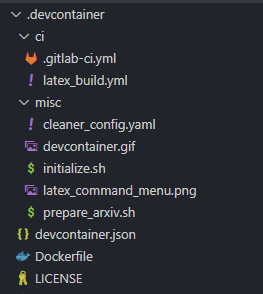
\includegraphics[width=.5\textwidth]{./images/image12.png}
	\caption{Visualizando o devcontainer pelo Visual Studio Code e dashboard do Docker}
	\label{fig:image12}
\end{figure}


Para esse projeto ser possíveloi necessária a utilização das mais variadas ferramentas de desenvolvimento:

- o github actions
- xu-cheng/latex-action@v2
- actions/upload-artifact@v3
- codespaces
- marvinpinto/actions
- site oficial da sbc
- docker
